\documentclass[a4paper,12pt]{article}
\usepackage[francais]{babel} % Package babel pour le français
\usepackage[T1]{fontenc}    % Package pour les accentuations
\usepackage[utf8]{inputenc}  % Français
\usepackage{textcomp}
\usepackage{lmodern}        % Pour avoir de bonnes polices en pdf
\usepackage{graphicx}       % Indispensable pour les figures
\usepackage{epstopdf}       % Utile pour les figures, résout une erreur
\usepackage{amsmath}        % Environnement pour les maths, permet du mettre du texte dans les équations
\usepackage{dialogue}		% Pour les dialogues
\usepackage{geometry}       % Utilisé pour les marges
\usepackage{pst-tree}		% Pour dessiner des arbres
\usepackage{pst-node}
\usepackage{multicol}		% Pour les colonnes
\usepackage{mathtools, bm}  % Typographie pour les ensembles communs
\usepackage{amssymb, bm}    % Typographie pour les ensembles communs
\usepackage{float}          % Pour bien placer les figures, scripts et tableaux
%\usepackage{listings}       % Utilisé pour les scripts
\usepackage{wrapfig}
\usepackage{xcolor}
\definecolor{vertclair}{rgb}{0.10,0.55,0.17}
\definecolor{vertfonce}{rgb}{0,0.44,0}
\definecolor{grisclair}{rgb}{0.78,0.78,0.78}
\definecolor{prune}{rgb}{0.65,0.00,0.00}
\definecolor{bleufonce}{rgb}{0.06,0.06,1.00}
\definecolor{violet}{rgb}{0.21,0.18,0.73}
\definecolor{orange}{rgb}{0.93,0.46,0.00}

\usepackage{tikz}			%Pour les figures et graphes
\usetikzlibrary{calc}		%Pour les figures et graphes
\usepackage[cache=false]{minted}        % Utilisé pour les scripts
\geometry{hmargin=3cm,vmargin=2cm} % Réglages des marges
\usepackage{fancyhdr}		% Pour l'entête et les pieds de page
\pagestyle{fancy}			% Pour l'entête et les pieds de page
\usepackage{hyperref}		% Pour les liens hypertext, sommaire et références
\usepackage[final]{pdfpages} % Pour inclure des .pdf

\renewcommand{\abstractname}{Avant-propos} %Modification du titre de l'abstract
\newcommand{\norme}[1]{\left\Vert #1\right\Vert} %Commande pour la norme euclidienne
\renewcommand{\listoflistingscaption}{Liste des programmes} %Pour changer le titre de la liste des codes
\renewcommand{\listingscaption}{Programme} %Pour changer la légende des codes
\newminted{console}{mathescape,
			   
               breaklines = true,
               numbersep=5pt,
               frame=lines,
               framesep=2mm}

\newminted{lisp}{mathescape,
			   
               breaklines = true,
               numbersep=5pt,
               frame=lines,
               framesep=2mm}

\renewcommand{\headrulewidth}{0.5pt}
\fancyhead[L]{IA01}
\fancyhead[R]{TP03 : Réalisation d’un système expert d’ordre $0+$}


\begin{document}


\thispagestyle{empty}

{\large

\vspace*{1cm}

\begin{center}

	{\bf Rapport de IA01 : \\Intelligence artificielle -- Représentation des connaissances}
	\vspace*{1cm}
	{\bf \\UNIVERSITE DE TECHNOLOGIE DE COMPIEGNE}

	\vspace*{1cm}
	
\includegraphics[scale=0.6]{UTC_logo.png}
	\vspace*{1cm}

	Automne 2016

	\vspace*{1cm}

	\vspace*{1cm}
	{\Large {\bf Guillaume JOUNEL \& Julien JERPHANION}}

	\vspace*{2 cm}
\end{center}

\flushleft{Sujet du rapport:\ \\
{\Large {\bf TP03 : Réalisation d’un système expert d’ordre $0+$}}}

\vspace*{1 cm}
\flushleft{Département des étudiants :\ \\
{\Large {\bf  Génie Informatique}}}\\

\vspace*{1 cm}
\flushleft{Professeur :\ \\
{\Large {\bf Marie-Hélène ABEL}}}\\
}

\newpage
\tableofcontents
%\newpage
%\listoffigures
\newpage
\listoflistings
\newpage

\section{Introduction : Présentation du système expert}


\subsection{Problématique}

Tous les programmeurs sont un jour confrontés au problème suivant :

\begin{quotation}
\centering
« \textit{Quels de programmation et technologies sont les plus adaptés pour le projet que je souhaite développer dans mon cadre d'utilisation ?} »
    
\end{quotation}


    Pour pallier à ce problème, nous allons concevoir un système expert qui propose différentes possibilités les plus adaptées selon l'usage.
    
    Pour cela, nous prendrons en compte de multiples critères tels que le domaine d'application (calcul numérique, intelligence artificielle...), l'expérience de l'utilisateur ou encore les caractéristiques de sa machine (Linux, MacOS...).
    
\subsection{Sources de connaissances sur le sujet}

    Les sources d'expertise ne manquent pas : il existe de nombreux sites et ressources sur le Net qui donnent les avantages et inconvénients de tous les langages de programmation existants selon les cas d'utilisation. En voici quelques uns :
    \begin{itemize}
        \item Wikipédia : Liste des langages de programmations par type :\\ \href{https://en.wikipedia.org/wiki/List_of_programming_languages_by_type}{\texttt{https://en.wikipedia.org/wiki/List\_of\_programming\_languages\_by\_type}} ;
        \item Learneroo: The Different Programming Languages :\\ \href{https://www.learneroo.com/modules/12/nodes/94}{\texttt{https://www.learneroo.com/modules/12/nodes/94}} ;
        \item WhoIsHostingThis: What Code Should You Learn?\\ \href{http://www.whoishostingthis.com/blog/2014/09/04/learn-to-code/}{\texttt{http://www.whoishostingthis.com/blog/2014/09/04/learn-to-code/}}.
    \end{itemize}


\subsection{Exemple d'intéraction}

Voici un exemple d'intéraction que l'on pourrait imaginer entre l'utilisateur et notre système :

\begin{dialogue}
    \speak{Syst\` eme} Spécificiez : Catégorie
    \speak{Utilisateur} [Application] --  Calcul scientifique -- Représentation de données
    \speak{Syst\` eme} Spécificiez : Type d'application
    \speak{Utilisateur} Système -- Web -- Jeu vidéo -- DIY -- [Applet] -- Application Smart-Phone -- Système Expert
    \speak{Syst\` eme}  Spécificiez : Usage
    \speak{Utilisateur} [Personnel] -- Réduit -- Universel
    \speak{Syst\` eme} Spécificiez : Niveau en Python
    \speak{Utilisateur} Excellent -- [Bon] -- Aucun
    \speak{Syst\` eme} Dans ce cas je vous conseille d'utiliser :
    \begin{itemize}
        \item \textbf{Python avec Tkinter} : permet de créer des interfaces graphiques (bibliothèque \texttt{Tk} ; plus d'information \href{https://wiki.python.org/moin/TkInter}{\textit{ici}} ;
        \item \textbf{Python avec Pygame} : adapté pour faire des petits jeux ; plus d'information \href{http://www.pygame.org/hifi.html}{\textit{ici}} ;
    \end{itemize}
\end{dialogue}


\subsection{Exemples de règles}

    Voici quelques idées pour de règles que l'on pourrait implémenter (\texttt{Technologies} est liste des propositions de solutions proposées en résultats par le système expert) :
    
    
    \begin{enumerate}
        \item     \texttt{SI (Catégorie = Application) ET (Type-application = Applet) ET\\ (Usage = Personnel) et (Niveau-Python = Bon) ALORS (Technologies = (Tkinter Pygame))}
        \item     \texttt{SI (Catégorie = Application) ET (Type-application = Web) ET\\ (Type-application-web = Statique) ET (Design = Aucun) ALORS\\\ (Technologies = (HTML5))}
        \item     \texttt{SI (Catégorie = Application) ET (Type-application = Système-Expert) ET (Intérêt = Pedagogique) ALORS (Technologies = (LISP Prolog))}
    \end{enumerate}
	
\section{Architecture}

\subsection{Base de règles}
Nous avons décidé d'implémenter notre base de règle de cette façon : 

\begin{listing}[H]
	\centering
	\inputminted[breaklines=true]{lisp}{../regles.lisp}
	\caption{Base de règles \texttt{*regles*}}
\end{listing}

\section{Base de faits \& Bases de connaissances}

Nous avons implémenté nos faits selon la forme suivante :

\begin{quotation}
	\texttt{(objet opérateur valeur)}
\end{quotation}

Pour donner les informations concernant les technologies choisies par \textit{Cactus} nous avons décider d'implémenter une base de connaissances. Celle-ci contient pour chaque technologie une brève description de celle-ci.

Les éléments des cette base sont représentés sous la forme de liste pointée ainsi :

\begin{quotation}
	\texttt{(technologie . "La description de la technologie")}
\end{quotation}

\begin{listing}[H]
	\centering
	\inputminted[breaklines=true]{lisp}{../technologies.lisp}
	\caption{Base de connaissances \texttt{*technologies*}}
\end{listing}

Nous utiliserons cette base de connaissances dans la fonction \texttt{afficherPropositions} que nous détaillerons plus bas.

\section{Fonctions outils}

\begin{listing}[H]
	\centering
	\inputminted[breaklines=true]{lisp}{../fonctionsOutils.lisp}
	\caption{Différentes fonctions outils}
\end{listing}
\[ \star \quad \star \quad \star \]

\newpage
%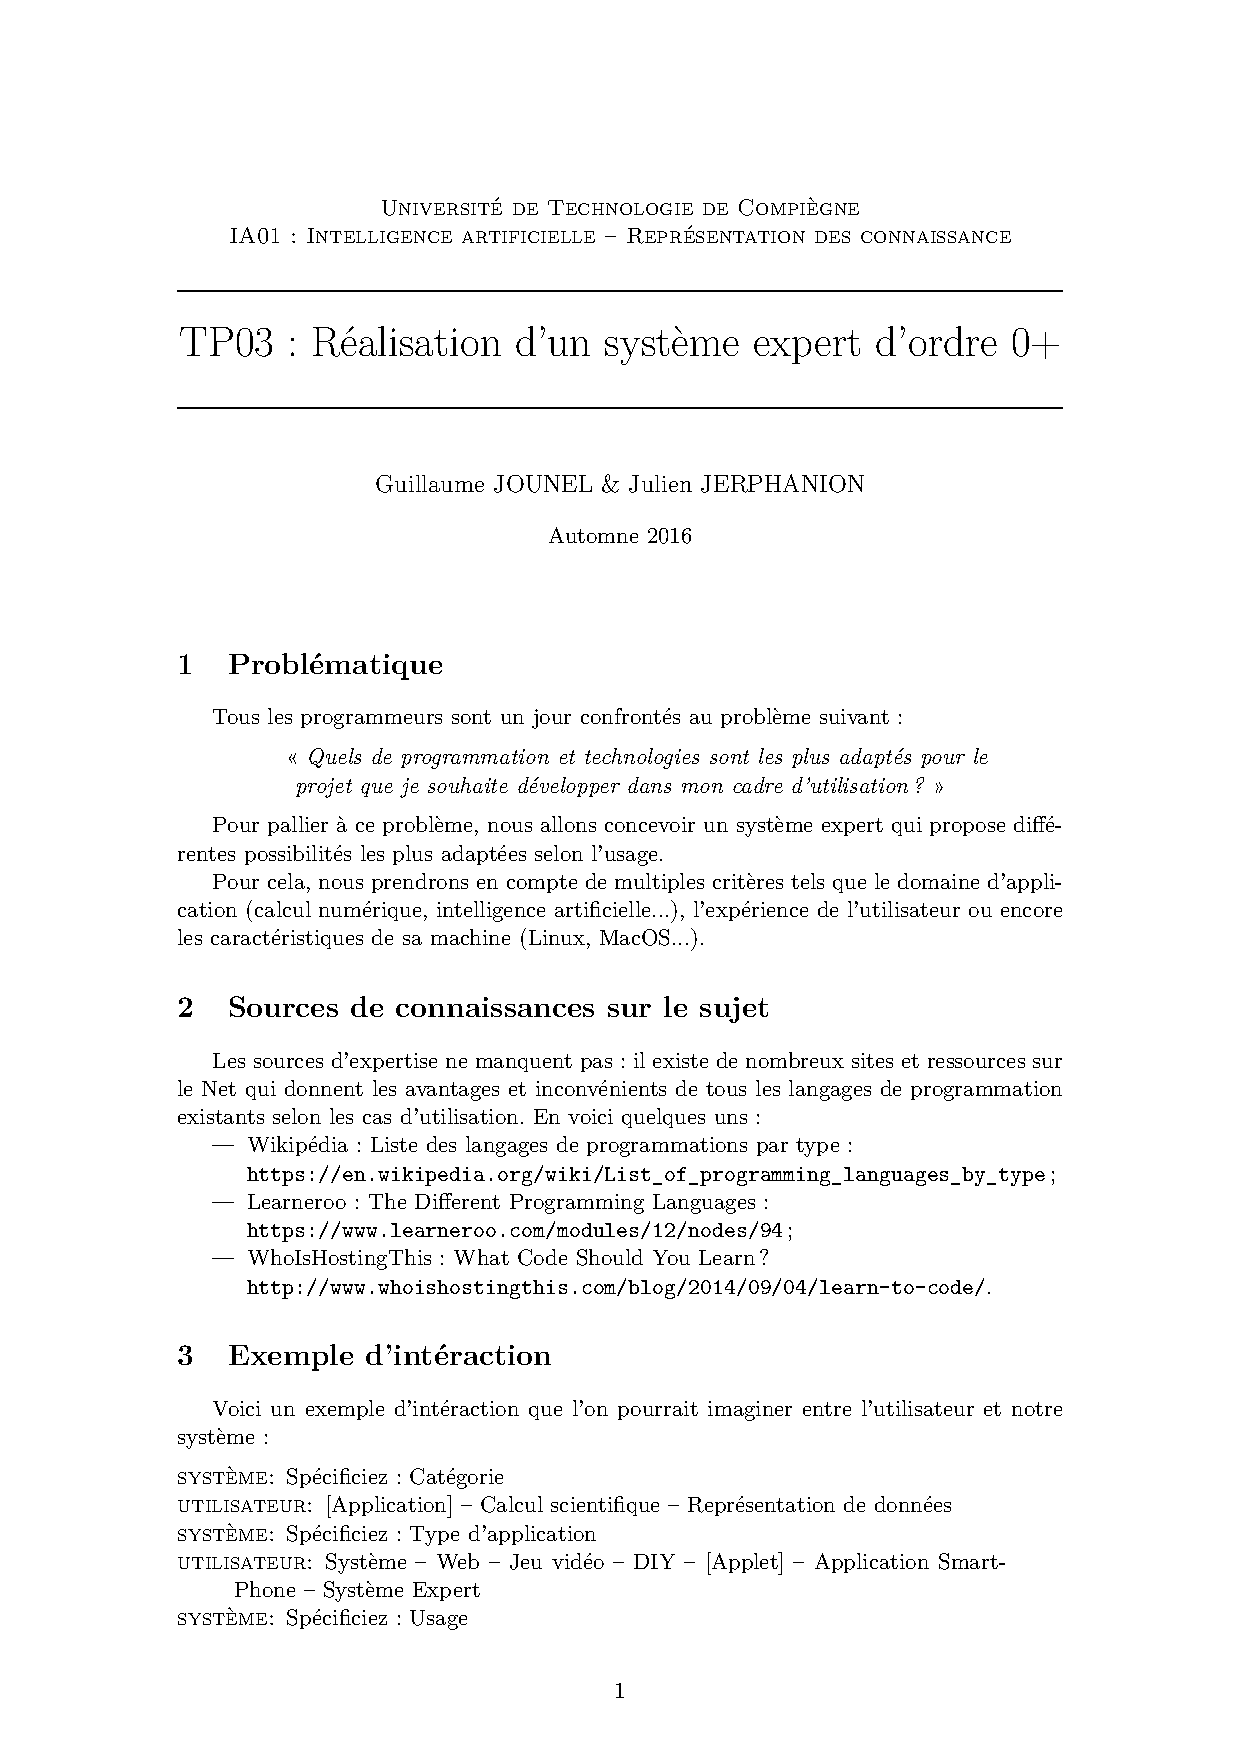
\includepdf[pages=1]{../sujetTP3.pdf}
\end{document}
	